\section{Описание}

В качестве датасета я выбрал \enquote{Heart Attack Analysis & Prediction Dataset} с сайта kaggle.\\
Он находится по ссылке https://www.kaggle.com/datasets/rashikrahmanpritom/heart-attack-analysis-prediction-dataset?select=heart.csv. \\В данном датасете собраны некоторые признаки, влияющие на возникновение сердечного приступа.\\

В этом наборе данных приведены признаки:\\

\begin{enumerate}
 \item Age : Возраст пациента
 \item Sex: Пол пациента
 \item exang: стенокардия, вызванная физической нагрузкой (1 = да; 0 = нет)
 \item cp: тип боли в груди
	\begin{enumerate}
	 \item Value 1: типичная стенокардия
	 \item Value 2: атипичная стенокардия
	 \item Value 3: неангинальная боль
	 \item Value 4: бессимптомное течение
	\end{enumerate}
 \item trtbps: артериальное давление в состоянии покоя (в мм рт. ст.)
 \item chol: холесторал в мг / дл, определяемый с помощью датчика ИМТ
 \item fbs: (уровень сахара в крови натощак> 120 мг / дл) (1 = истина; 0 = ложь)
 \item rest\_ecg : результаты электрокардиографии в состоянии покоя
	\begin{enumerate}
	 \item Value 0: нормальное
	 \item Value 1: аномалия зубца ST-T (инверсия зубца T и / или повышение или понижение ST> 0,05 мВ)
  	 \item Value 2: отображение вероятной или определенной гипертрофии левого желудочка по критериям Эстеса
	\end{enumerate}
 \item thalach: достигнутая максимальная частота сердечных сокращений
 \item target : 0 = меньше шансов сердечного приступа 1 = больше шансов сердечного приступа
\end{enumerate}




\pagebreak

\section{Ход работы}

Сначала проверим датасет на наличие в нем пустых ячеек, с помощью info().
Таковых там не оказалось.

\begin{alltt}
RangeIndex: 303 entries, 0 to 302
Data columns (total 14 columns):
 \#   Column    Non-Null Count  Dtype  
---  	------    	--------------  		-----  
 0   age       	303 non-null    	int64  
 1   sex       	303 non-null    	int64  
 2   cp        	303 non-null    	int64  
 3   trtbps    	303 non-null    	int64  
 4   chol      	303 non-null    	int64  
 5   fbs       	303 non-null    	int64  
 6   restecg   	303 non-null    	int64  
 7   thalachh   303 non-null    	int64  
 8   exng      	303 non-null    	int64  
 9   oldpeak    303 non-null    	float64
 10  slp       	303 non-null    	int64  
 11  caa       	303 non-null    	int64  
 12  thall     	303 non-null    	int64  
 13  output     303 non-null    	int64  
dtypes: float64(1), int64(13)
memory usage: 33.3 KB
\end{alltt}

Так как все данные записаны в численном виде, мне не пришлось придумывать, как символьным данным сопоставить числа.\\
Дальше я проверил существуют ли повторяющиеся строки и если существуют, то дублирующаяся строка удаляется.

\begin{lstlisting}[language=C]
print(data.shape)
\end{lstlisting}

\begin{alltt}
(303, 14)
\end{alltt}

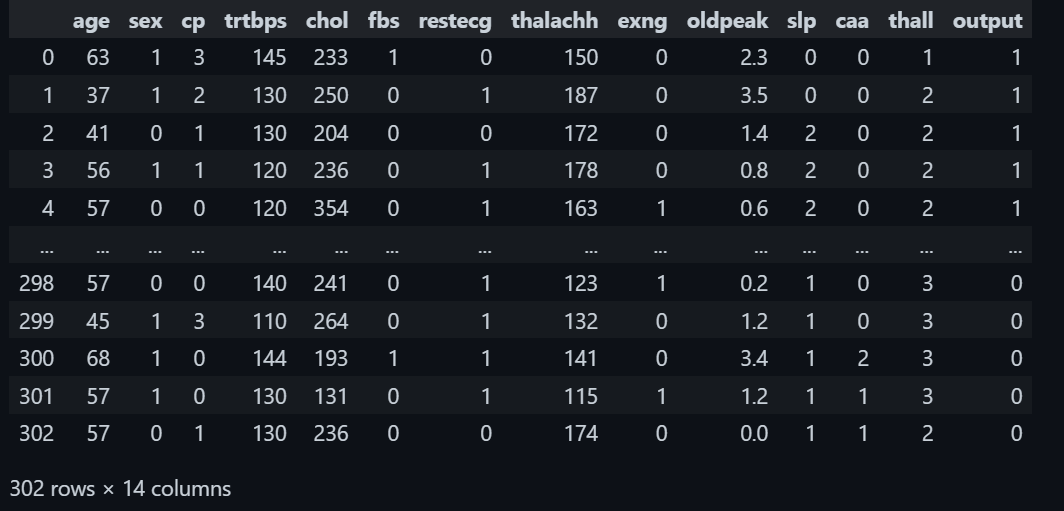
\includegraphics[width=\textwidth]{Table}

Далее я перешел непосредственно к анализу зависимостей в данных, построил корреляционную матрицу.

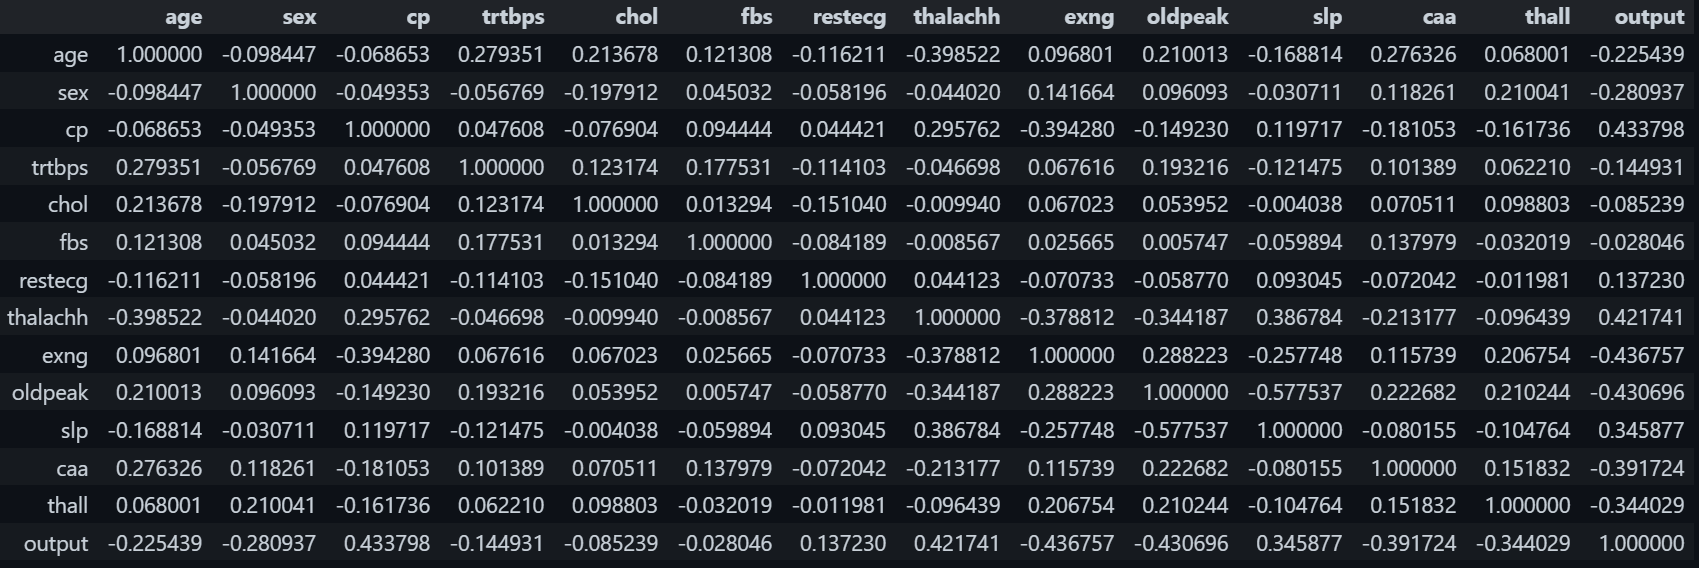
\includegraphics[width=\textwidth]{corrMatrix}

Далее я построил тепловую карту корреляционной матрицы.

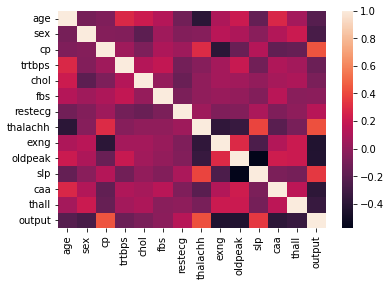
\includegraphics[width=\textwidth]{heatMap} 

Так как целевым параметром является параметр output (0 = меньше вероятность сердечного приступа 1 = больше вероятность сердечного приступа) проанализируем последнюю колонку или строку.  Из матрицы видно, что больше всего на этот параметр влияют: тип боли в груди (cp), достигнутая максимальная частота сердечных сокращений (thalachh), стенокардия, вызванная физической нагрузкой  (exng), подавление сегмента ST, вызванное упражнением относительно отдыха. (oldpeak).
А меньше
всего - холесторал в мг / дл (chol) и уровень сахара в крови натощак (fbs). Также из матрицы видно, что
остальные параметры сильно между собой некоррелируют, следовательно, можно не
удалять/объединять их.
Дальше я рассмотрел параметры моих признаков в датасет

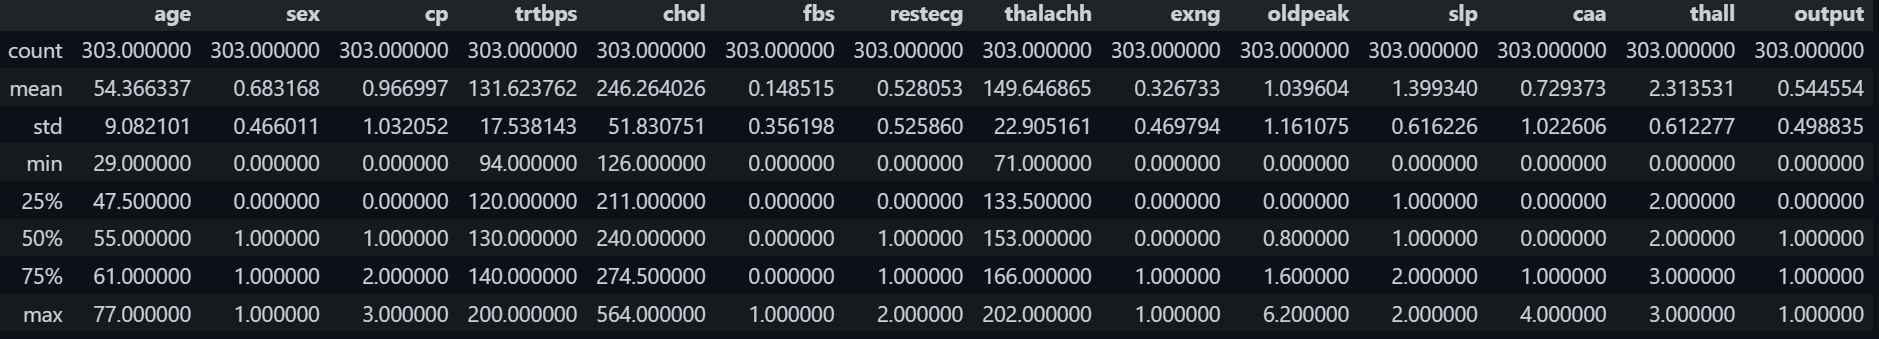
\includegraphics[width=\textwidth]{normalizTable} 

\pagebreak

Отсюда видно, что данные ненормированы. Придется это иправить по мере реализации
модели. Также можно подтвердить, что данные находятся в указанных диапазонах,
как и говорится в описании к датасету\\

Далее построим гистаграммы распределения признаков. Для колличественных построим графики, где по оси X указывается значение параметра, а по Y - его количество

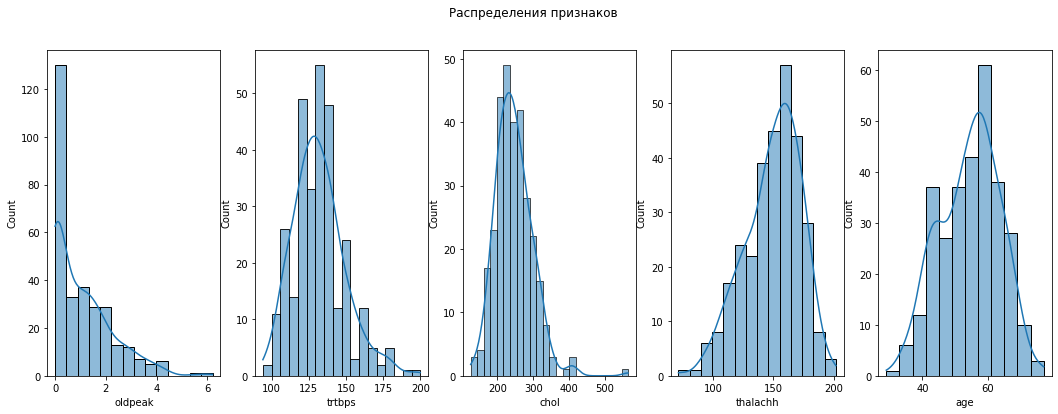
\includegraphics[width=\textwidth]{gist} 

Из графиков видно, что значения распределены неравномерно, но эти распределения
похожи на нормальные. Также на данных гистаграммах мной не были замечены выбросы, следовательно никаких изменений в датасет вносить не надо.\\

Также на графике oldpeak видно, что много людей с ST = 0, что является патологией. Скорее
всего, датасет был основан на людях с больным сердцем, это косвено подтверждает возраст указанный в выборке. Все пациенты из датасета в примерно попадают в диапазон от 40 до 60 лет\\

\pagebreak

Далее построим диаграммы для категориальных признаков.

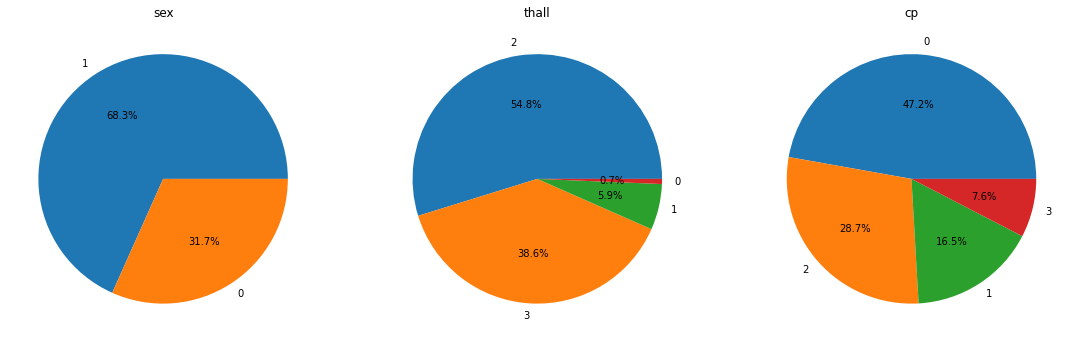
\includegraphics[width=\textwidth]{diagram1} 

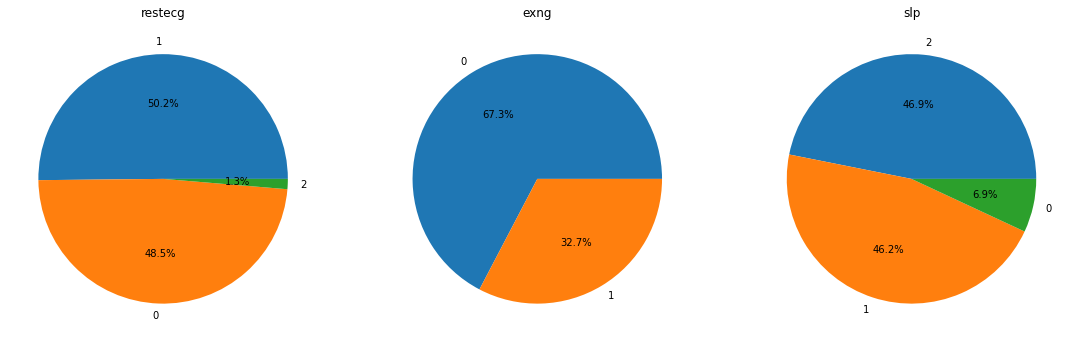
\includegraphics[width=\textwidth]{diagram2} 

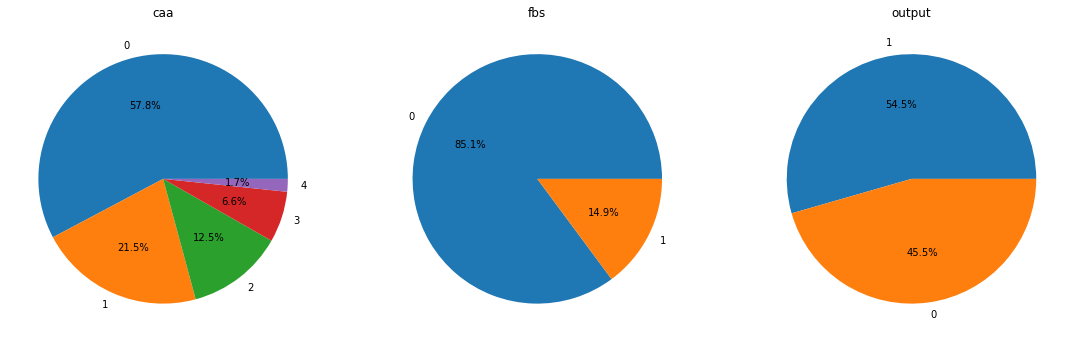
\includegraphics[width=\textwidth]{diagram3} 

Из данных диаграмм видно, что данные распределены неравномерно. Из диаграммы outout видно, что больных и здоровых людей примерно поровну, так что оверсемплинг делать не требуется.\\

Построим парные графики, при этом выделим цветом данные параметра HeartDisease.


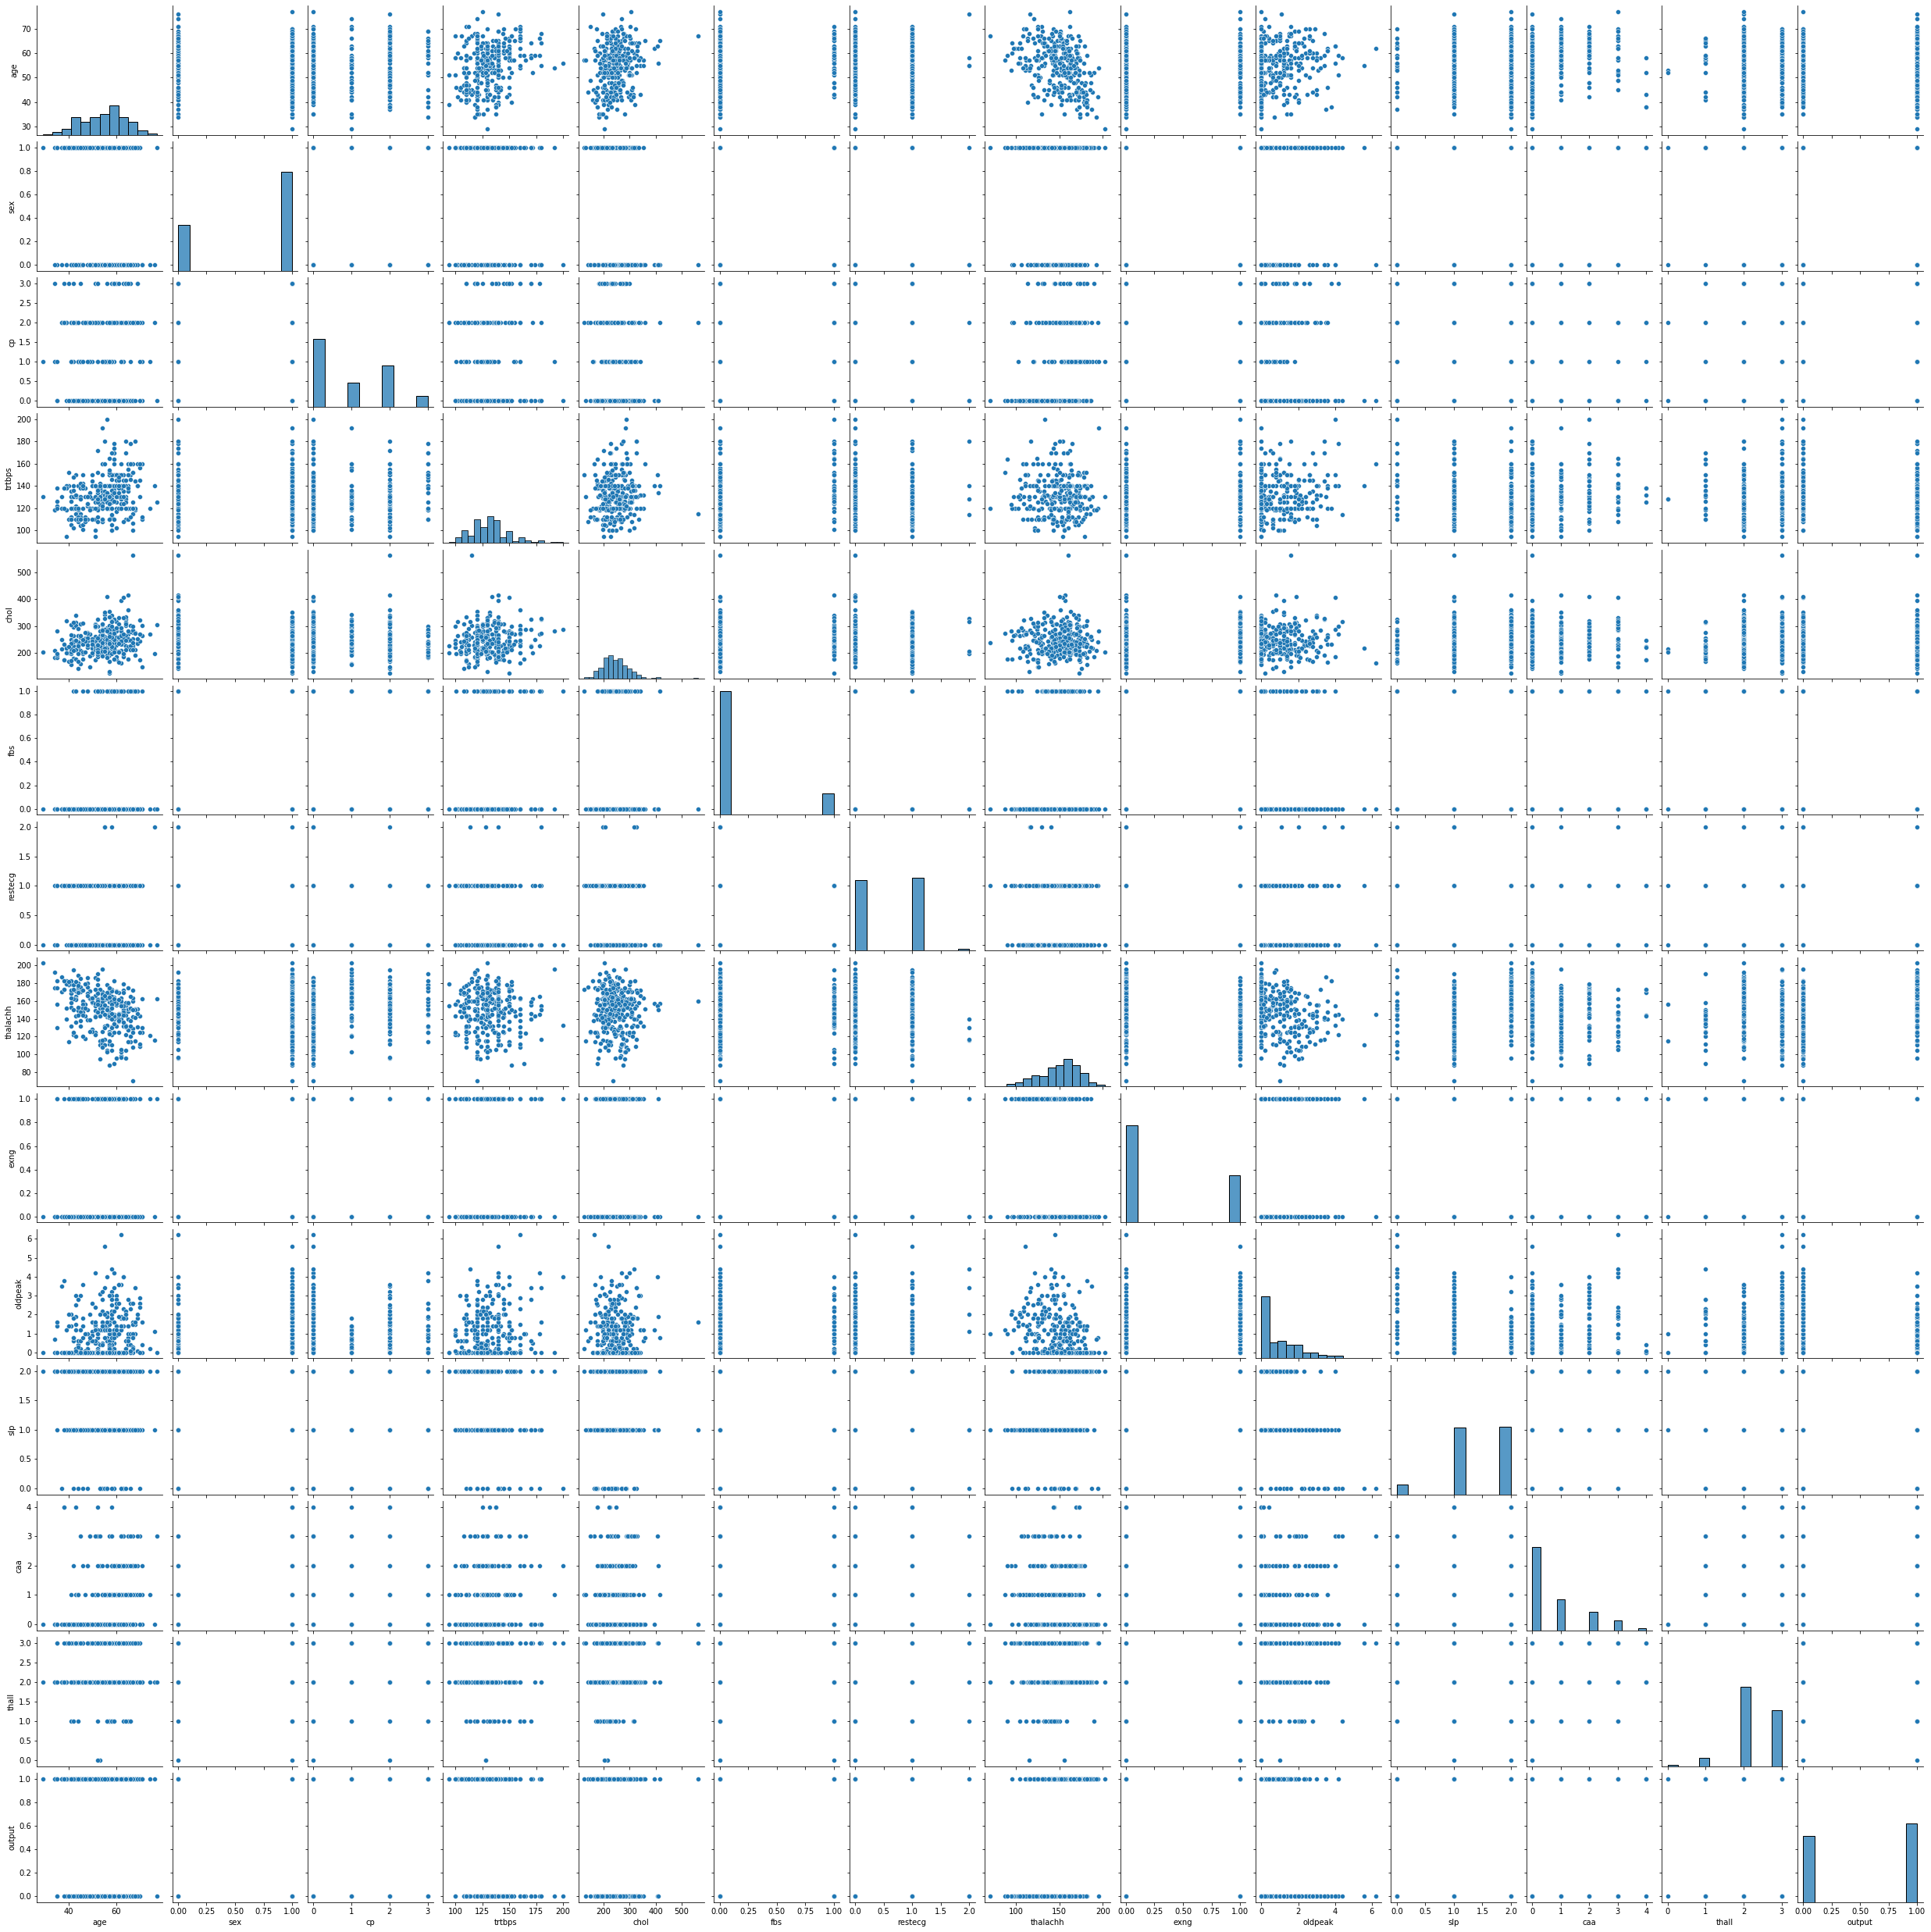
\includegraphics[width=\textwidth]{corrGraph} 

Данные распределены достаточно хаотично. Добавлять новые признаки не требуется. Данные готовы
к обучению.


\pagebreak